\documentclass[tikz]{standalone}
\usetikzlibrary{bayesnet, arrows.meta}

\begin{document}
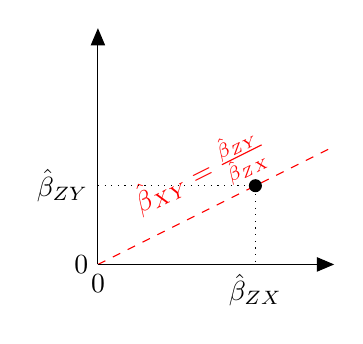
\begin{tikzpicture}
\coordinate (origin) at (0,0);
\coordinate (ZX) at (3,0);
\coordinate (ZY) at (0,3);
%\node (ZX) at (3,0) {$\beta_{ZX}$};
%\node (ZY) at (0,3) {$\beta_{ZY}$};

\coordinate (ZXhat) at (2,0);
\path (ZXhat) node[below] {$\hat{\beta}_{ZX}$};
\coordinate (ZYhat) at (0,1);
\path (ZYhat) node[left] {$\hat{\beta}_{ZY}$};

\draw[red,dashed] (origin) -- node[sloped,above] {$\hat{\beta}_{XY} = \frac{\hat{\beta}_{ZY}}{\hat{\beta}_{ZX}}$} (3, 1.5);

\draw[dotted] (ZYhat) -| node[circle,fill,solid,scale=0.5] {} (ZXhat);
\path (origin) node[below] {0} (origin) node[left] {0};
\path[->] (origin) edge (ZX);
\path[->] (origin) edge (ZY);
\end{tikzpicture}
\end{document}
